\section{CLIO Pocket}
Til selve målingerne blev der brugt en såkaldt \textbf{CLIO Pocket}. Dette er et værktøj som er i stand til, at måle både frekvenskarakteristikker og impulsresponser.

\begin{wrapfigure}{r}{0.5\textwidth} 
	\vspace{-20pt}
	\begin{center}
		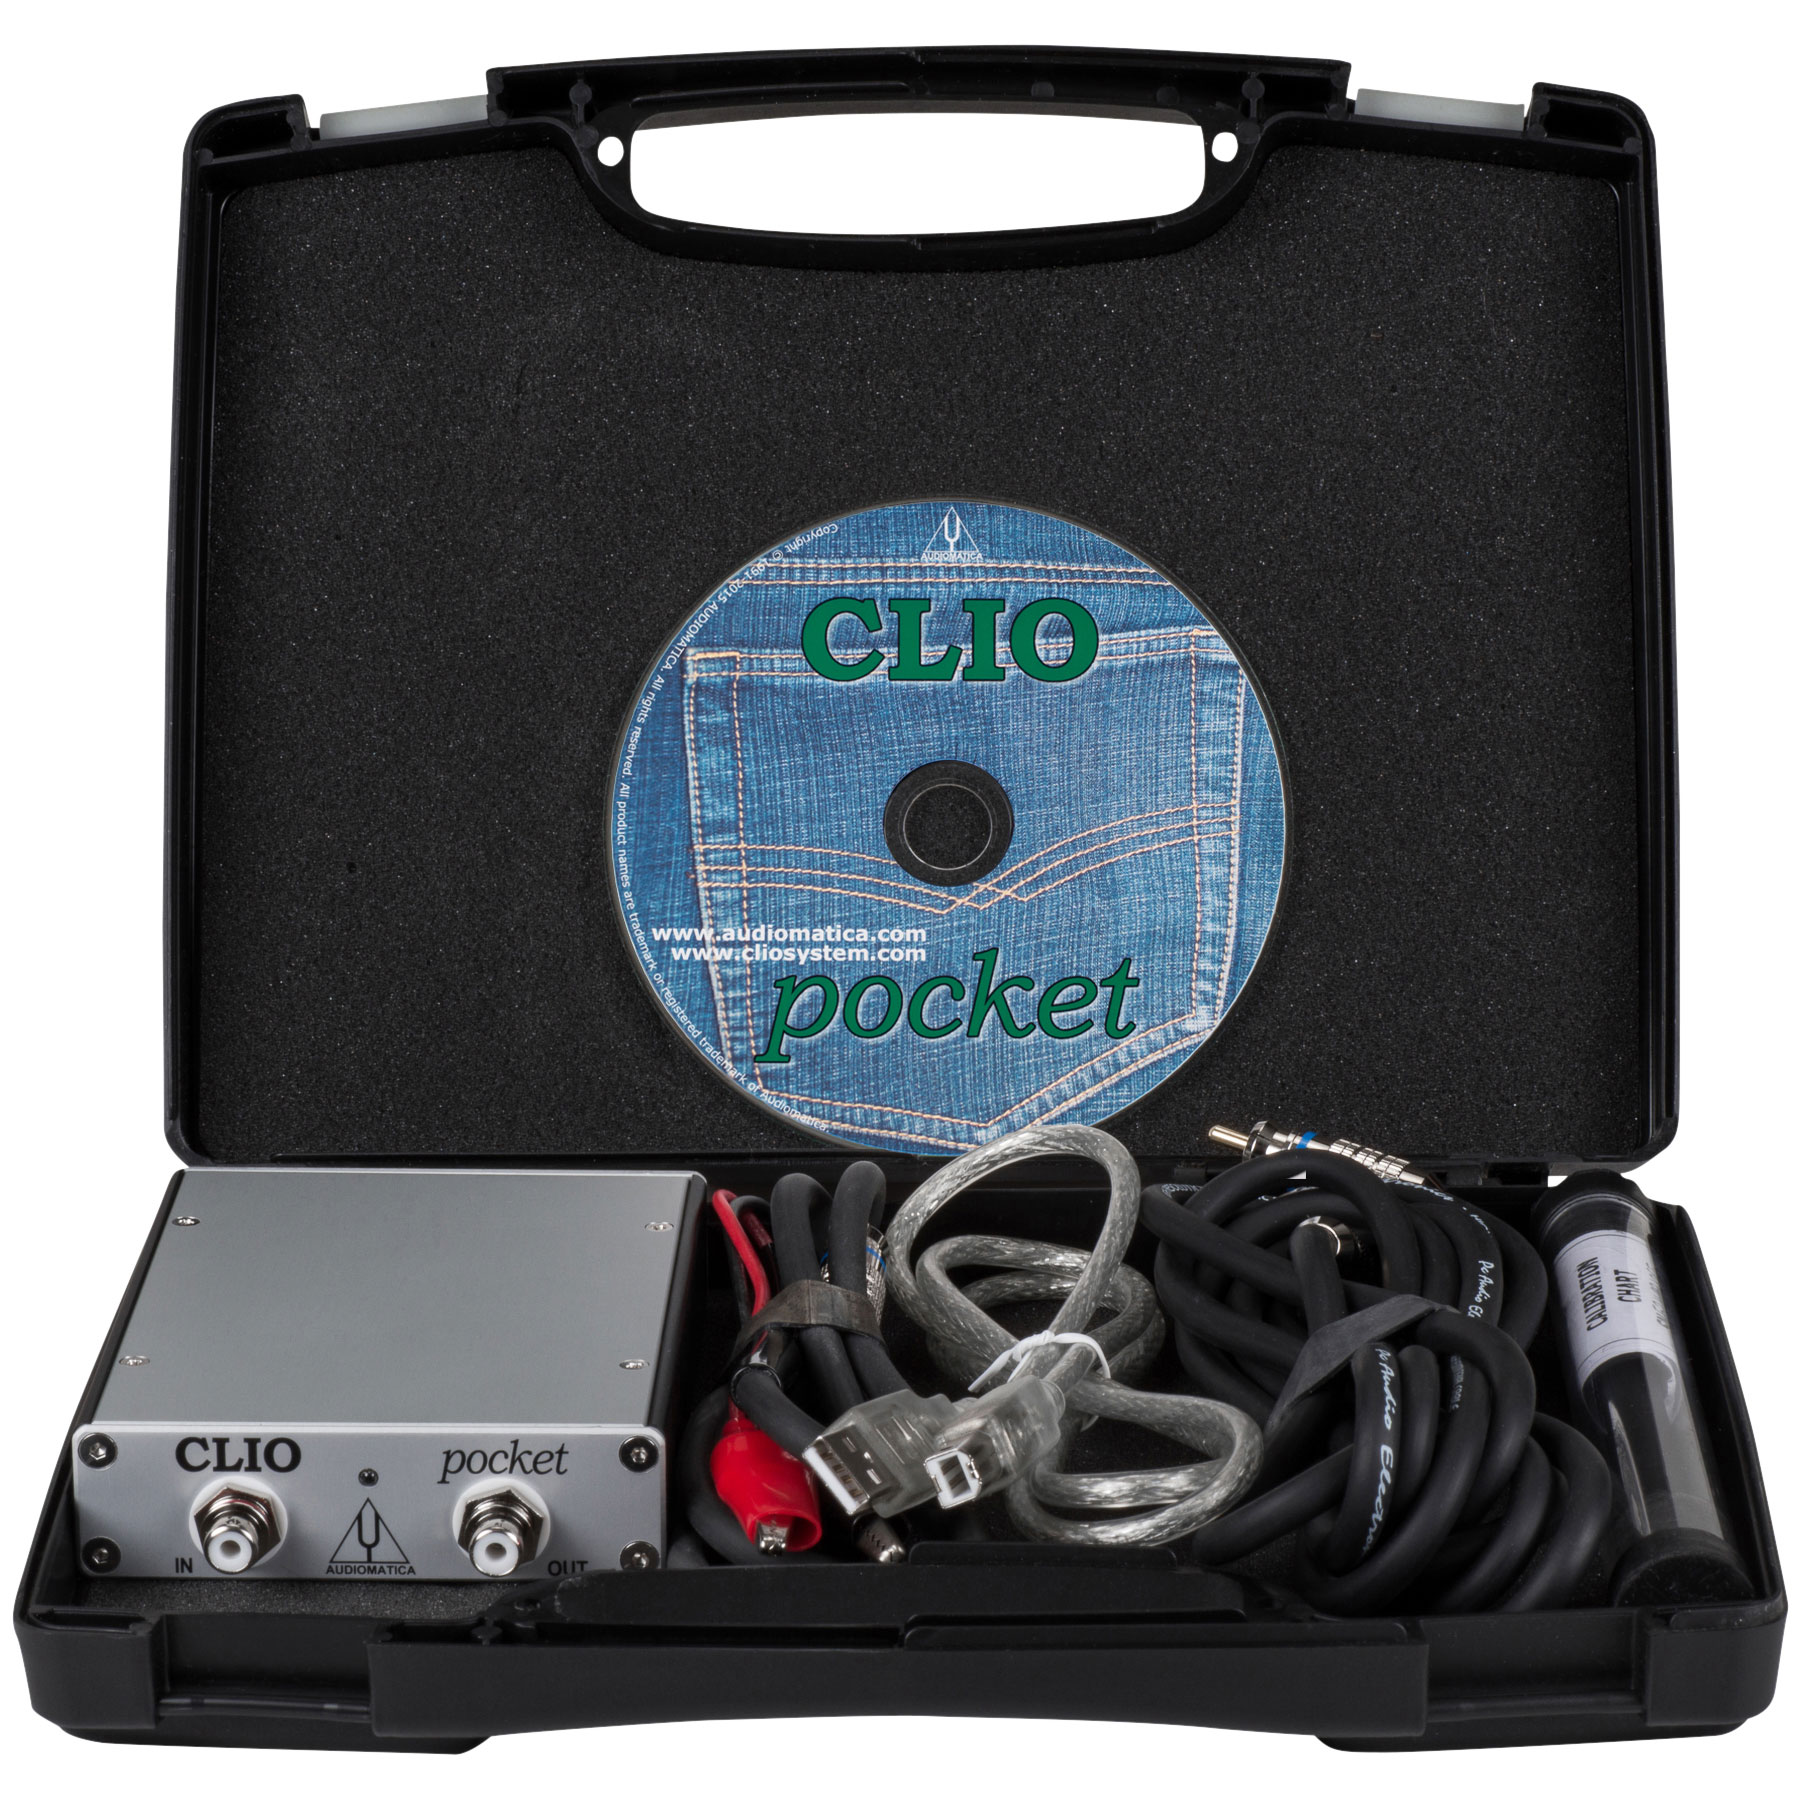
\includegraphics[width=0.4\textwidth]{Billeder/ClioPocket}
	\end{center}
	\caption{CLIO Pocket}
	\vspace{-20pt}
\end{wrapfigure}
Selve modulet har en indgang som sluttes til en mikrofon og en udgang som sluttes til en højtaler. Derudover findes der en USB-forbindelse til tilslutning til en computer.

Værktøjet måler en frekvenskarakteristik ved, at udsende to frekvenschirps efter hinanden gennem højtaleren som så måles igen af mikrofonen. Disse måleresultater bruges så til, at udarbejde en frekvenskarakteristik i området fra \SI{10}{\hertz} til \SI{20}{\kilo\hertz}.

Den målemetode som CLIO Pocket benytter sig af kan derfor beskrives gennem en simpel feedback-løkke svarende til det, som er vist på diagrammet nedenfor.

Som vist på diagrammet, så vil højtalerens udformning (membran og refleks), rummets udformning og mikrofonens karakteristika alle have en betydning for det målte frekvensrespons. I de målinger der fremkommer i denne rapport er det dog blevet antaget, at mikrofonens karakteristika kun har en minimal betydning. 

\begin{figure}[H]
	\centering
	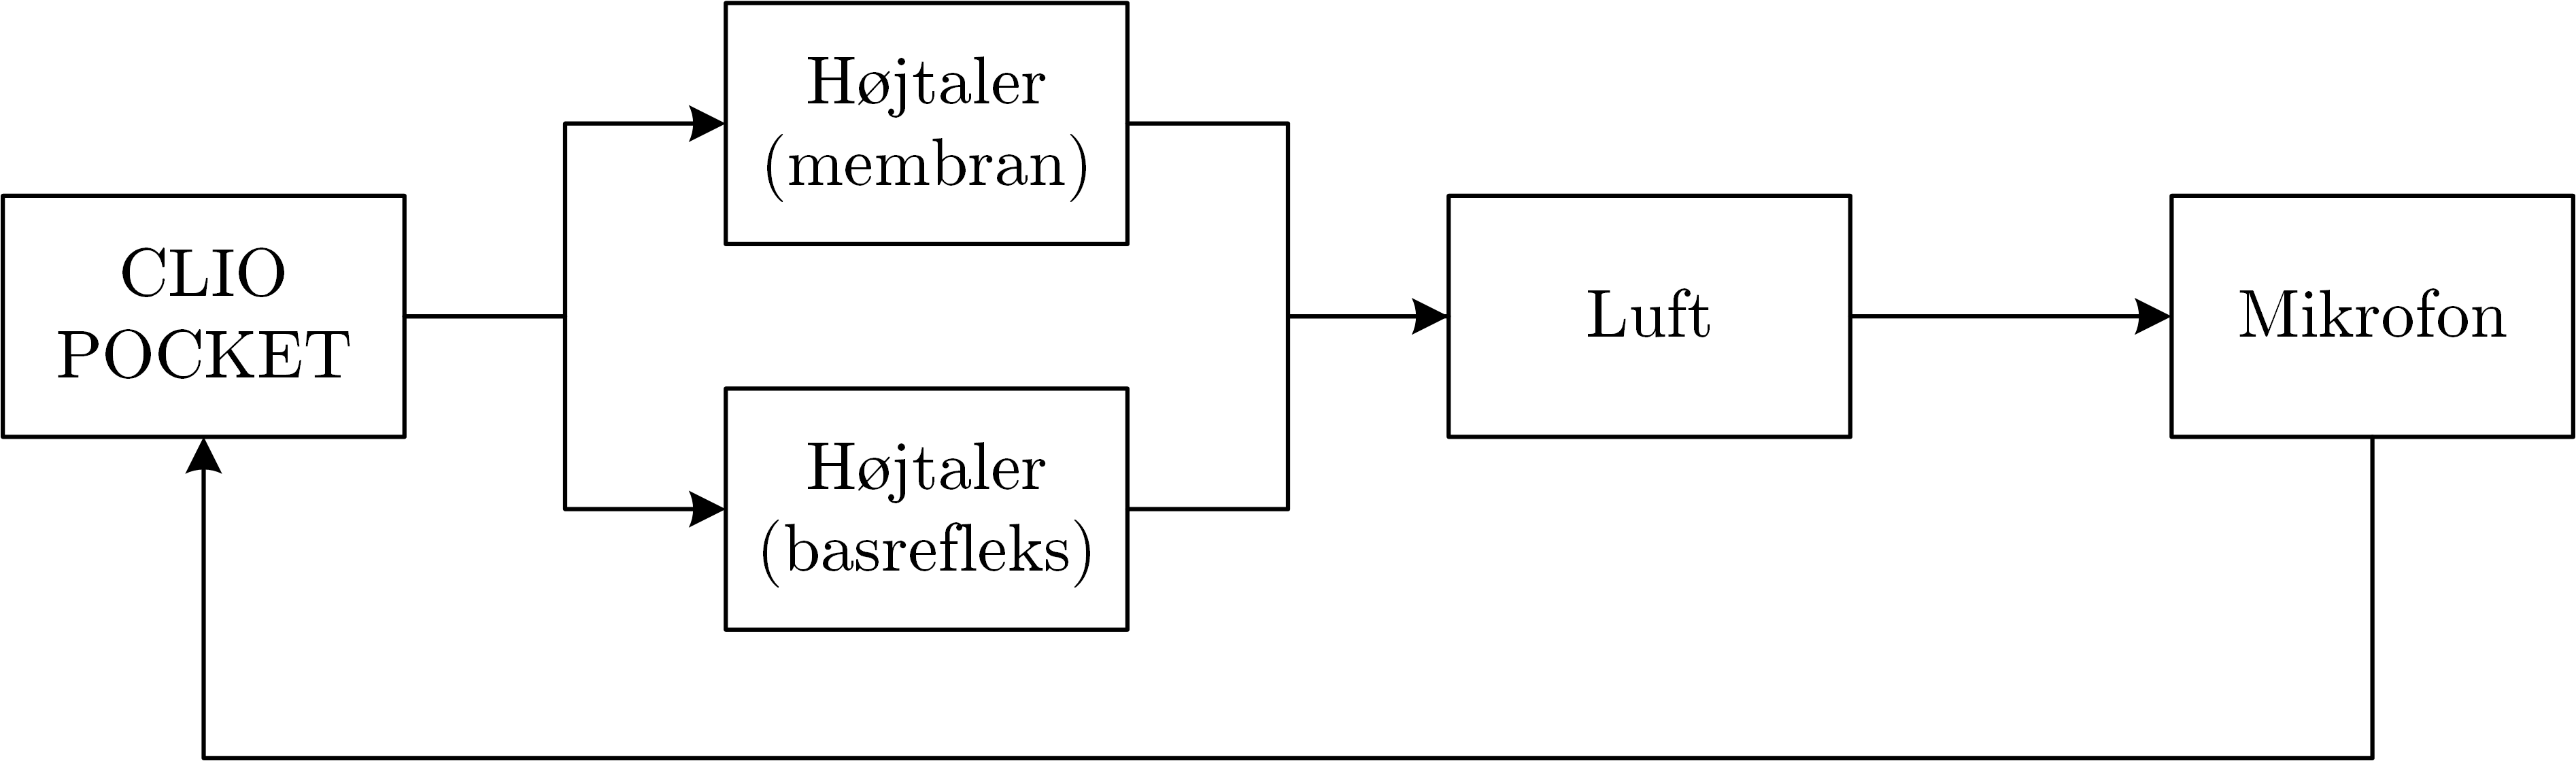
\includegraphics[width=\textwidth]{Billeder/CLIOFeedback}
	\caption{CLIO Pocket målemetode}
	\label{fig:ClioFeedback}
\end{figure}